\chapter{Dynamic Pipeline Framework in Haskell}\label{dp-hs}
One of the fundamental piece of the present work as we have described in ~\autoref{intro} and ~\autoref{prelim},
is the design and implementation of \acrfull{dpfh}: a \acrshort{dpf} written in \acrshort{hs} which allow \acrshort{hs} users
to implement any suitable algorithm in \acrshort{dp}, providing the correct abstractions that helps on that matter.

During the process of conducting this research, we have implemented \acrshort{dpfh}~\cite{dynamic-pipeline} and publishes it into \acrfull{hack}~\cite{hackage}.
In this chapter, we are going to describe the design and implementation details of \acrshort{dpfh}.

\section{Framework Design}

\subsection{Background}
Any suitable framework should provide the user the right level of abstraction that removes and hides enough complexity, 
to allow the developer to focus on the problem that needs to be solved.
There are several design approximations to implement a framework: \begin{inparaenum}[i\upshape)]
  \item  \emph{Configuration Based} where the user only 
  focuses on completing specific configuration files and provides them to the framework's runtime system to execute the program,
  \item  \emph{Convention over Configuration (CoC)} where the user writes his code and definition following certain patterns in naming or source disposition 
  and the framework interprets from that, what is the execution flow that needs to be done,
  \item \emph{Application Programing Interface (API)} where the framework or library provides a certain amount
  of functionality implemented in terms of functions or interfaces, and the user needs to compose those functions or implement those abstractions to achieve the desired results, and finally
  \item \emph{\acrfull{dsl}} where the framework or library provides a new language that represents the domain problem and allows to program the solution in terms of that high-level language. 
   \end{inparaenum}.

In the \acrfull{dsl} approach~\cite{dsl} there exists two types of it: \acrfull{dsl} and \acrfull{edsl}. \acrshort{dsl}, usually called external \acrshort{dsl}, the propose is to create a completely new language with its own semantic, syntax, and interpreter. 
In general, these languages are not general-purpose languages, because as their name indicates, they are domain-specific. On the other hand, \acrshort{edsl} are syntactically embedded in the host language of the library, and the user writes on it but is restricted by the abstractions provided by the \acrshort{edsl}.
\acrshort{dpfh} follows a \acrshort{edsl} approach taking advantage of the strong type \acrshort{hs} system giving the user correctness proof at type-level.

\subsection{Architectural Design}
In this section we are going to focus on the architectural design of the \acrshort{dpfh} using a \acrshort{edsl} approach. We have built a framework that contains
three important components: \acrshort{dsl}, \acrshort{idl} and \acrshort{rs}. 

\begin{figure}[!ht]
  \centering
  \begin{minipage}{\textwidth}
   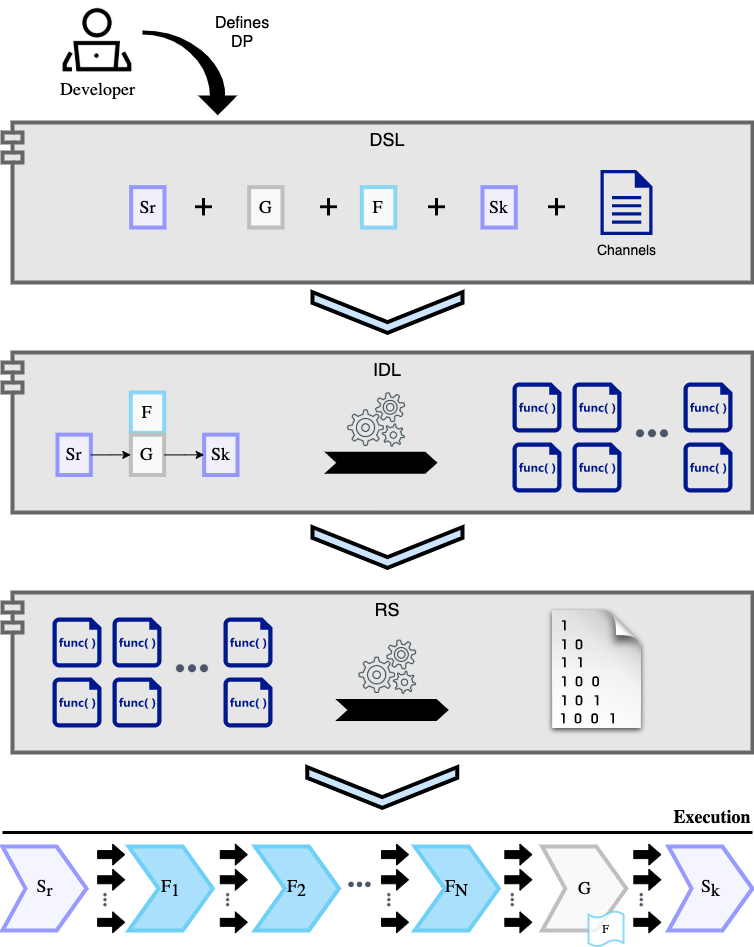
\includegraphics[width=1\textwidth, height=0.6\textheight]{dpf_haskell_v3.png}
    \caption{Architectural view of \acrshort{dpfh}}
    \label{fig:dpfh:1}
  \end{minipage}
\end{figure}

In \autoref{fig:dpfh:1} we can appreciate the different components mentioned before that are the grey boxes.

\paragraph{DSL} The user interacts with the \acrshort{dsl} component where defines how the \acrshort{dp} disposition
should be, and what are the channels that are going to communicate the stages of the pipeline. For example, in the
case of \autoref{prole} that we develop the \acrshort{wcc} algorithm, the user knows that is going to receive from the Standard Input 
the edges of the graph and therefore, two channels are needed between $\iwcc$, $\gwcc$ and $\owcc$, one for sending the edges and another for sending
the accumulated connected components. 

\paragraph{IDL} Based on the definition provided in the \acrshort{dsl}, the user interacts with the \acrshort{idl} which guides him/her to build the functions with the algorithms needed for each stage: $\iwcc$, $\gwcc$, $\owcc$, $\fwcc$, and actors. 

\paragraph{RS} Once we have the \acrshort{dp} definition and the functions provided by the user with the algorithm solution, the framework
can be fed with these components to execute the program using the \acrshort{rs}. 

\section{Implementation}
In this section, we describe the details of all the techniques used for implementing each architectural layer described before.
As we have explained in \autoref{sec:contrib}, this library was published on Hackage~\cite{dynamic-pipeline}, the source code is open and can be found on this Github Repository~\cite{dynamic-pipeline-git}.

\subsection{DSL Grammar}\label{sub:sec:dsl-gram}
In order to provide a Type-safe verification in compilation time, we have defined a \acrfull{cfg} that generates a \acrshort{dp} \acrshort{dsl} language and it is encoded in custom types. 
This allows the user to define a type-level \acrshort{dp} of the pipeline he wants to build. 

\begin{definition}[\acrshort{dsl} \acrshort{cfg}]
Lets have the grammar $\gdsl = (N, \Sigma, DB, P)$, where $N$ is the set of non-terminal symbols, $\Sigma$ the set of terminal symbols,
$DP \in N$ is the start symbol and $P$ are the generation rules, such that:
\begin{equation*}
    \boxed{
      \begin{aligned}
    N &= \{DP,S_r,S_k,G,F_b,CH,CH_s\},\\
    \Sigma &= \{\text{\mintinline{haskell}{Source}},\text{\mintinline{haskell}{Generator}},\text{\mintinline{haskell}{Sink}},\text{\mintinline{haskell}{FeedbackChannel}},\text{\mintinline{haskell}{Type}},\text{\mintinline{haskell}{Eof}},\text{\mintinline{haskell}{:=>}},\text{\mintinline{haskell}{:<+>}}\},
    \end{aligned}
    }
\end{equation*}
\begin{equation*}
  \boxed{
    \begin{aligned}
  P = \{\\
  DP  &\rightarrow S_r\ \text{\mintinline{haskell}{:=>}}\ G\ \text{\mintinline{haskell}{:=>}}\ S_k\ |\ S_r\ \text{\mintinline{haskell}{:=>}}\ G\ \text{\mintinline{haskell}{:=>}}\ F_b\ \text{\mintinline{haskell}{:=>}}\ S_k,\\
  S_r &\rightarrow \text{\mintinline{haskell}{Source}}\ CH_s,\\
  G   &\rightarrow \text{\mintinline{haskell}{Generator}}\ CH_s,\\
  S_k &\rightarrow \text{\mintinline{haskell}{Sink}},\\
  F_b &\rightarrow \text{\mintinline{haskell}{FeedbackChannel}} CH,\\
  CH_s &\rightarrow \text{\mintinline{haskell}{Channel}}\ CH,\\
  CH &\rightarrow \text{\mintinline{haskell}{Type :<+>}}\ CH\ |\ \text{\mintinline{haskell}{Eof}}\}
\end{aligned}
}
\end{equation*}
\end{definition}

In order to encode this on the language, we need an Index type~\cite{type-index} to keep track of the information, at type-level, that we do not want to lose, and it is needed for generating the \acrshort{dp}. 
In that sense, we create an Index type for each element $e$, such that $e \in \Sigma$.

\begin{listing}[H]
  \begin{minted}[fontsize=\small,numbers=left,breaklines,frame=lines,framerule=2pt,framesep=2mm,baselinestretch=1.2,highlightlines={3,4}]{haskell}

data Source (a :: Type)
data Generator (a :: Type)
data Sink
data Eof
data Channel (a :: Type)
data FeedbackChannel (a :: Type)

  \end{minted}
  \caption{[\mintinline{shell}{Flow.hs}] $\Sigma$ enconding of $G_{dsl}$}
  \label{src:dpfh:1}
\end{listing}
  
As we can see in \autoref{src:dpfh:1}, highlighted types are terminal symbols of $\gdsl$ that are not indexed with any Index type. 
This is because they do not carry any extra type of information that we need to remember. In the case of \mintinline{haskell}{Sink}, since it is the last stage that does not connect further with any other stage, we do not need to indicate channel information. 
\mintinline{haskell}{Eof} it is just a terminal type to disambiguate the \mintinline{haskell}{Channel (a :: Type)} subtree of the full parser tree. Since \mintinline{haskell}{Channel} can carry any type, 
because we need to allow a different number of channels and channels types, we need a symbol that marks the end of the channel list.

There are two more important symbols $e \in \Sigma$ that need to be addressed independently: \mintinline{haskell}{:=>} and \mintinline{haskell}{:<+>}.

\begin{listing}[H]
  \begin{minted}[fontsize=\small,numbers=left,breaklines,frame=lines,framerule=2pt,framesep=2mm,baselinestretch=1.2,highlightlines={1,5}]{haskell}

data chann1 :<+> chann2 = chann1 :<+> chann2
  deriving (Typeable, Eq, Show, Functor, Traversable, Foldable, Bounded)
infixr 5 :<+>
   
data a :=> b = a :=> b
  deriving (Typeable, Eq, Show, Functor, Traversable, Foldable, Bounded)
infixr 5 :=>
   
  \end{minted}
  \caption{[\mintinline{shell}{Flow.hs}] $\Sigma$ enconding of $G_{dsl}$ - Especial non-terminals}
  \label{src:dpfh:2}
\end{listing}

In \autoref{src:dpfh:2}, \mintinline{haskell}{:=>} and \mintinline{haskell}{:<+>} can combine 2 types. 
These types are syntactic sugar for writing the \acrshort{dsl} \acrshort{cfg}. 
Apart from that, they are different because we need two distinguishable symbols $e \in \Sigma$, to separate the encoding of the pipeline stage ($\iwcc$, $\gwcc$, $\owcc$)
from the encoding of channel composition in the same stage, as we can appreciate in the $\gdsl$ definition.

As an user, and having this few type setup, we can start defining our pipelines.  
For example, if we want to generate a language for \acrshort{dp} that eliminates duplicated in a stream, we know that we only need one channel connecting the stages that carry out the type, in this case, \mintinline{haskell}{Int}.

\begin{listing}[H]
  \begin{minted}[fontsize=\small,numbers=left,breaklines,frame=lines,framerule=2pt,framesep=2mm,baselinestretch=1.2,highlightlines={}]{haskell}

type DPExample = Source (Channel (Int :<+> Eof)) 
              :=> Generator (Channel (Int :<+> Eof)) 
              :=> Sink
   
  \end{minted}
  \caption{Example of \acrshort{dp} encoded in $G_{dsl}$}
  \label{src:dpfh:3}
\end{listing}

\subsection{DSL Validation}\label{sub:sec:dsl-val}
The language generated by the grammar needs to be validated in order to avoid the user makes mistakes and provide an incorrect \acrshort{dp} definition.
Fortunately, \acrshort{hs} provides several Type-level techniques~\cite{type-haskell} which allows us to verify properties of our programs in the language before running it, 
saving the users to write bugs and eliminates errors. This verification done by the compiler is establishing a Curry-Howard Isomorphism~\cite{curryhoward}: 
\emph{Propositions as Types - Programs as Proof}.\footnote{Although \acrshort{hs} is not a theorem prover System like Coq~\cite{coq}, some verifications as we are showing in this work can be done with the compiler to obtain some proof about our programs.}

Although \acrshort{hs} provides a lot of tools to build a type correspondence with propositional logic that can be check at compilation type, it is also known that all these
techniques require the addition of \emph{Haskell Language Extensions}. We cannot forget that even though \acrshort{hs} has more than 20 years of 
Academic Research on its core language, some of the features has been added as extensions, especially the ones that implement state of the art Type Theory concepts. 

The first thing to remark, according to the definition on the previous \autoref{sub:sec:dsl-gram}, is the validation of the grammar. 
In order to validate the \acrshort{dsl} \acrshort{cfg} at type-level we use a \emph{Associated Type Family}~\cite{associated-types}.


\begin{listing}[H]
  \begin{minted}[fontsize=\small,numbers=left,breaklines,frame=lines,framerule=2pt,framesep=2mm,baselinestretch=1.2,highlightlines={6,18}]{haskell}

type family And (a :: Bool) (b :: Bool) :: Bool where
    And 'True 'True = 'True
    And a b         = 'False
  

type family IsDP (dpDefinition :: k) :: Bool where
    IsDP (Source (Channel inToGen) :=> Generator (Channel genToOut) :=> Sink)
        = And (IsDP (Source (Channel inToGen))) (IsDP (Generator (Channel genToOut)))
    IsDP ( Source (Channel inToGen) :=> Generator (Channel genToOut) :=> FeedbackChannel toSource :=> Sink)
        = And (IsDP (Source (Channel inToGen))) (IsDP (Generator (Channel genToOut)))
    IsDP (Source (Channel (a :<+> more)))     
        = IsDP (Source (Channel more))
    IsDP (Source (Channel Eof))               = 'True
    IsDP (Generator (Channel (a :<+> more)))  = IsDP (Generator (Channel more))
    IsDP (Generator (Channel a))              = 'True
    IsDP x                                    = 'False
     
type family ValidDP (a :: Bool) :: Constraint where
  ValidDP 'True = ()
  ValidDP 'False = TypeError
                    ( 'Text "Invalid Semantic for Building DP Program"
                      ':$$: 'Text "Language Grammar:"
                      ':$$: 'Text "DP       -> Source CHANS :=> Generator CHANS :=> Sink"
                      ':$$: 'Text "DP       -> Source CHANS :=> Generator CHANS :=> FEEDBACK :=> Sink"
                      ':$$: 'Text "CHANS    -> Channel CH"
                      ':$$: 'Text "FEEDBACK -> FeedbackChannel CH"
                      ':$$: 'Text "CH       -> Type :<+> CH | Eof"
                      ':$$: 'Text "Example: 'Source (Channel (Int :<+> Int)) :=> Generator (Channel (Int :<+> Int)) :=> Sink'"
                    )
  \end{minted}
  \caption{[\mintinline{shell}{Stage.hs}] Validating encoded in $G_{dsl}$ - FCF}
  \label{src:dpfh:4}
\end{listing}

Types in \acrshort{hs} are fully applied and \mintinline{haskell}{IsValid} type, as we see in \autoref{src:dpfh:4}, needs to generate the language
of the grammar providing evidence to the Type System that the user must define that language and no other is possible. 
\mintinline{haskell}{IsValid} Type Family fully applies to a \mintinline{haskell}{Bool} promoted Type~\cite{promoted-types} (not a boolean value), \mintinline{haskell}{'True} or 
\mintinline{haskell}{'False}. With this technique and defining a custom type-level error, defined in \mintinline{haskell}{ValidDP} type, the compiler will help the user to verify that the definition generates the correct language.
Now we can use these Types to constraint functions and ensure the user definition will be type-checked by the compiler.

\begin{listing}[H]
  \begin{minted}[fontsize=\small,numbers=left,breaklines,frame=lines,framerule=2pt,framesep=2mm,baselinestretch=1.2,highlightlines={2}]{haskell}

mkDP :: forall dpDefinition filterState filterParam st.
    ( ValidDP (IsDP dpDefinition)
    , DPConstraint dpDefinition filterState st filterParam)
 => Stage (WithSource dpDefinition (DP st)) 
 -> GeneratorStage dpDefinition filterState filterParam st  
 -> Stage (WithSink dpDefinition (DP st))  
 -> DP st ()
mkDP = ...

someFunc = mkDP @DPExample ...

  \end{minted}
  \caption{Using validation of \acrshort{dp} encoded in $G_{dsl}$}
  \label{src:dpfh:5}
\end{listing}

Other details will be cover later in this chapter, but in \autoref{src:dpfh:5} we can appreciate how we can restrict the function using
the type family defined. Only with that, the compiler will show an error if the \acrshort{dp} definition is not correct.

\subsection{\acrfull{idl}}
\acrshort{idl} component takes the definition made on with \acrshort{dsl} grammar to interpret and generate the function definitions
that the user needs to fill in for solving a specific problem. In \autoref{sec:dp}, we have described what the user needs to provide in a \acrshort{dp} algorithm: $\iwcc$, $\gwcc$, $\owcc$, and the $\fwcc$ with the non-empty set of Actors.

The \acrshort{idl} generates the function definitions with an empty implementation completed by the user, ensuring that those functions will give Proof of the Propositions defined on the \acrshort{dsl}, therefore there is a Curry-Howard Correspondence~\cite{curryhoward}.

Similar techniques that we used on \autoref{sub:sec:dsl-val} are also used here. On the first hand, we again use type-level \emph{Type-level Defunctionalization}~\cite{defunctionalization, fun-type-function-haskell} technique to 
let the compiler generates the signatures of the required functions and then a Term level \emph{Defunctionalization} to interpret that functions.
At the same time, Type Index~\cite{type-index} and Heterogeneous List~\cite{hlist} are used to keep track of the dynamic number and parameters types of each 
function. 

\begin{listing}[H]
  \begin{minted}[fontsize=\small,numbers=left,breaklines,frame=lines,framerule=2pt,framesep=2mm,baselinestretch=1.2,highlightlines={2,6,10}]{haskell}

withSource :: forall (dpDefinition :: Type) st. WithSource dpDefinition (DP st) 
            -> Stage (WithSource dpDefinition (DP st))
withSource = mkStage' @(WithSource dpDefinition (DP st))

withGenerator :: forall (dpDefinition :: Type) (filter :: Type) st. WithGenerator dpDefinition filter (DP st) 
              -> Stage (WithGenerator dpDefinition filter (DP st))
withGenerator = mkStage' @(WithGenerator dpDefinition filter (DP st))

withSink :: forall (dpDefinition :: Type) st. WithSink dpDefinition (DP st) 
           -> Stage (WithSink dpDefinition (DP st))
withSink = mkStage' @(WithSink dpDefinition (DP st))
  \end{minted}
  \caption{[\mintinline{shell}{Stage.hs}] Using withXXXX Interpreters of \acrshort{dp} encoded in $G_{dsl}$}
  \label{src:dpfh:6}
\end{listing}

As we can see on \autoref{src:dpfh:6} there is \mintinline{haskell}{Stage *} class type that encodes term-level \emph{Defunctionalization}, and that class is polymorphic in the type of Stage it can build.
The differents \mintinline{haskell}{WithSource}, \mintinline{haskell}{WithGenerator} and \mintinline{haskell}{WithSink}
\emph{Associated Type Families}~\cite{associated-types} help the compiler to deduce the signature of the function that the user should provide for that Stage.


\begin{listing}[H]
  \begin{minted}[fontsize=\small,numbers=left,breaklines,frame=lines,framerule=2pt,framesep=2mm,baselinestretch=1.2,highlightlines={7,11}]{haskell}

type family WithSource (dpDefinition :: Type) (monadicAction :: Type -> Type) :: Type where
  WithSource (Source (Channel inToGen) :=> Generator (Channel genToOut) :=> Sink) monadicAction
      = WithSource (ChanIn inToGen) monadicAction
  WithSource (Source (Channel inToGen) :=> Generator (Channel genToOut) :=> FeedbackChannel toSource :=> Sink) monadicAction 
      = WithSource (ChanOutIn toSource inToGen) monadicAction
  WithSource (ChanIn (dpDefinition :<+> more)) monadicAction         
      = WriteChannel dpDefinition -> WithSource (ChanIn more) monadicAction
  WithSource (ChanIn Eof) monadicAction                              
      = monadicAction ()
  WithSource (ChanOutIn (dpDefinition :<+> more) ins) monadicAction  
      = ReadChannel dpDefinition -> WithSource (ChanOutIn more ins) monadicAction
  WithSource (ChanOutIn Eof ins) monadicAction                       
      = WithSource (ChanIn ins) monadicAction
  WithSource dpDefinition _                                          
      = TypeError
          ( 'Text "Invalid Semantic for Source Stage"
            ':$$: 'Text "in the DP Definition '"
            ':<>: 'ShowType dpDefinition
            ':<>: 'Text "'"
            ':$$: 'Text "Language Grammar:"
            ':$$: 'Text "DP       -> Source CHANS :=> Generator CHANS :=> Sink"
            ':$$: 'Text "DP       -> Source CHANS :=> Generator CHANS :=> FEEDBACK :=> Sink"
            ':$$: 'Text "CHANS    -> Channel CH"
            ':$$: 'Text "FEEDBACK -> FeedbackChannel CH"
            ':$$: 'Text "CH       -> Type :<+> CH | Eof"
            ':$$: 'Text "Example: 'Source (Channel (Int :<+> Int)) :=> Generator (Channel (Int :<+> Int)) :=> Sink'"
          )
  \end{minted}
  \caption{[\mintinline{shell}{Stage.hs}] WithSource Associate Type Details}
  \label{src:dpfh:7}
\end{listing}

In \autoref{src:dpfh:7} we can see in the highlighted lines how the type induction is expanding a function definition of the form \mintinline{haskell}{a -> b -> ...} depending on \acrshort{dp} language definition. 
Let's see how \mintinline{haskell}{Stage} was defined in order to read saturate this type and ask the user the proper function according to that generated type.

\begin{listing}[H]
  \begin{minted}[fontsize=\small,numbers=left,breaklines,frame=lines,framerule=2pt,framesep=2mm,baselinestretch=1.2,highlightlines={12,16}]{haskell}

data Stage a where
  Stage :: Proxy a -> a -> Stage a

mkStage' :: forall a. a -> Stage a
mkStage' = Stage (Proxy @a)
    
  \end{minted}
  \caption{[\mintinline{shell}{Stage.hs}] Stage Data Type}
  \label{src:dpfh:8}
\end{listing}

As we can see in \autoref{src:dpfh:8}, it is using a simple \mintinline{haskell}{Proxy a} from \mintinline{haskell}{Data.Proxy} phantom type technique, to remember the type definition generated by \mintinline{haskell}{a}.
In the case of \mintinline{haskell}{withSource} interpreter shown in \autoref{src:dpfh:6}, \\
$\mintinline{haskell}{a} \thicksim \mintinline{haskell}{WithSource definition}$, where $\thicksim$ means isomorphic. Therefore 
when compiler fully applies the type it can tell the user what is the function that \mintinline{haskell}{Stage} should contain.

\paragraph{Generator and Filter}
Generator ($\gwcc$) and Filter ($\fwcc$) should be explained together because as we have seen on \acrshort{dp} definition in \autoref{sec:dp},
$\gwcc$ has a $\fwcc$ template in order to know how to dynamically interpose a new $\fwcc$ during the runtime execution of the program.
Let's first study $\fwcc$ Data Type in the context of the framework.

\begin{listing}[H]
  \begin{minted}[fontsize=\small,numbers=left,breaklines,frame=lines,framerule=2pt,framesep=2mm,baselinestretch=1.2,highlightlines={2,5}]{haskell}

newtype Actor dpDefinition filterState filterParam monadicAction =
    Actor {  unActor :: MonadState filterState monadicAction => Stage (WithFilter dpDefinition filterParam monadicAction) }

newtype Filter dpDefinition filterState filterParam st =
    Filter { unFilter :: NonEmpty (Actor dpDefinition filterState filterParam (StateT filterState (DP st))) }
    deriving Generic
    
  \end{minted}
  \caption{[\mintinline{shell}{Stage.hs}] Filter / Actor Data Type}
  \label{src:dpfh:9}
\end{listing}

$\fwcc$ is a \mintinline{haskell}{NonEmpty} list of \mintinline{haskell}{Actor}. This exactly represents the same as the \acrshort{dp} theoretical definition.
It is important to highlight from this \autoref{src:dpfh:9} the following concepts. 
On the first hand, an \mintinline{haskell}{Actor} is a \mintinline{haskell}{Stage}, which is obvious since it is the \mintinline{haskell}{NonEmpty Actor} list the final unit of execution (a.k.a. Stage), and therefore what is going to interpose between the $\gwcc$ and the previous Filters. 
Moreover \mintinline{haskell}{Actor} Stage is defunctionalized with \mintinline{haskell}{WithFilter} \emph{Associated type family} with the same concept as we have seen before for the other stages. 
Because of this, the user of the framework will be able to generate the actor functions (proof) that need to provide to the framework, according to the language definition.
On the other hand, \mintinline{haskell}{Filter} wraps an explicit \mintinline{haskell}{StateT} monadic context. This is because the $\fwcc$ instance should have an state, by \acrshort{dp} definition in \autoref{sec:dp}.
For example, in the case of $\dpwcc$, as we have seen in \autoref{prole} $\fwcc$ keeps an updated list of connected components that are updated as long as it receives more edges that are connected with the current list.
Finally, some combinators and smart constructors are provided in the framework to facilitate the construction of $\fwcc$ and Actors as we can see in \autoref{src:dpfh:10}.

\begin{listing}[H]
  \begin{minted}[fontsize=\small,numbers=left,breaklines,frame=lines,framerule=2pt,framesep=2mm,baselinestretch=1.2,highlightlines={}]{haskell}

mkFilter :: forall dpDefinition filterState filterParam st. WithFilter dpDefinition filterParam (StateT filterState (DP st)) 
         -> Filter dpDefinition filterState filterParam st
mkFilter = Filter . single

single :: forall dpDefinition filterState filterParam st. WithFilter dpDefinition filterParam (StateT filterState (DP st)) 
       -> NonEmpty (Actor dpDefinition filterState filterParam (StateT filterState (DP st)))
single = one . actor

actor :: forall dpDefinition filterState filterParam st. WithFilter dpDefinition filterParam (StateT filterState (DP st)) 
      -> Actor dpDefinition filterState filterParam (StateT filterState (DP st))
actor = Actor . mkStage' @(WithFilter dpDefinition filterParam (StateT filterState (DP st)))

(|>>>) :: forall dpDefinition filterState filterParam st. Actor dpDefinition filterState filterParam (StateT filterState (DP st)) 
       -> Filter dpDefinition filterState filterParam st 
       -> Filter dpDefinition filterState filterParam st
(|>>>) a f = f & _Wrapped' %~ (a <|)
infixr 5 |>>>

(|>>) :: forall dpDefinition filterState filterParam st. Actor dpDefinition filterState filterParam (StateT filterState (DP st)) 
      -> Actor dpDefinition filterState filterParam (StateT filterState (DP st)) 
      -> Filter dpDefinition filterState filterParam st
(|>>) a1 a2 = Filter (a1 <|one a2)
infixr 5 |>>
  \end{minted}
  \caption{[\mintinline{shell}{Stage.hs}] Filter / Actor smart constructors and combinators}
  \label{src:dpfh:10}
\end{listing}

Now in the following \autoref{src:dpfh:11}, we can see $\gwcc$ containing a $\fwcc$ template that we have explained before and its own stage behavior.

\begin{listing}[H]
  \begin{minted}[fontsize=\small,numbers=left,breaklines,frame=lines,framerule=2pt,framesep=2mm,baselinestretch=1.2,highlightlines={}]{haskell}
data GeneratorStage dpDefinition filterState filterParam st = GeneratorStage
    { _gsGenerator      :: Stage (WithGenerator dpDefinition (Filter dpDefinition filterState filterParam st) (DP st))
    , _gsFilterTemplate :: Filter dpDefinition filterState filterParam st
    }  
  \end{minted}
  \caption{[\mintinline{shell}{Stage.hs}] Generator}
  \label{src:dpfh:11}
\end{listing}

\subsection{\acrfull{rs}}
The \acrshort{rs} can be divided into two parts: the combinators that allow in runtime generate stages dynamically, as long as data arrives at $\gwcc$,
and the execution context of the \acrshort{dp}.

Regarding execution context, all the stages that we have seen in previous sections are the pieces needed to build an executable \mintinline{haskell}{DP st a} monad.
This executable monad has an existential type similar to \mintinline{haskell}{ST} monad to not escape out from the context on different stages.

Once the dynamic pipeline starts to execute, the core of the framework dynamically generates stages between $\gwcc$ and previous stages, according to the user definition. 
This is not more than an \emph{anamorphism}~\cite{lenses} that creates $\fwcc$ instance until some condition is met.

\begin{listing}[H]
  \begin{minted}[fontsize=\small,numbers=left,breaklines,frame=lines,framerule=2pt,framesep=2mm,baselinestretch=1.2,highlightlines={2,12,14,15,16,17,18}]{haskell}
unfoldF :: forall dpDefinition readElem st filterState filterParam l. SpawnFilterConstraint dpDefinition readElem st filterState filterParam l
        => UnFoldFilter dpDefinition readElem st filterState filterParam l 
        -> DP st (HList l) 
unfoldF = loopSpawn

where
  loopSpawn uf@UnFoldFilter{..} =
    maybe (pure _ufRsChannels) (loopSpawn <=< doOnElem uf) =<< DP (pull _ufReadChannel)

  doOnElem uf@UnFoldFilter{..} elem' = do
    _ufOnElem elem'
    if _ufSpawnIf elem'
     then do
       (reads', writes' :: HList l3) <- getFilterChannels <$> DP (makeChansF @(ChansFilter dpDefinition))
       let hlist = elem' .*. _ufReadChannel .*. (_ufRsChannels `hAppendList` writes')
       void $ runFilter _ufFilter (_ufInitState elem') hlist (_ufReadChannel .*. (_ufRsChannels `hAppendList` writes'))
       return $ uf { _ufReadChannel = hHead reads', _ufRsChannels = hTail reads' }
     else return uf

  \end{minted}
  \caption{[\mintinline{shell}{Stage.hs}] unfoldF}
  \label{src:dpfh:12}
\end{listing}

In \autoref{src:dpfh:12} the \mintinline{haskell}{unfoldF} receives an \mintinline{haskell}{UnFoldFilter} Data type, which contains the recipe for controlling that unfold recursive call. 
In line 12, \mintinline{haskell}{_ufSpawnIf} and field of \mintinline{haskell}{UnFoldFilter}, indicates when to stop the recursion. 
Inside the conditional, in the first line, we create new channels for that filter because we need to create new channels for connecting this new filter computation with the previous and with the next. 
Therefore, the next stage is going to be fed with the new channels of this new filter. After that, we run the filter to put the computation 
to work in the pipeline, and finally, we return the new channels to the next stage, which is going to be $\gwcc$.
As we can also be appreciated in the code, there is an intensive use of \mintinline{haskell}{HList}~\cite{hlist}. This is because since the \acrshort{dp}
definition made by the user dynamically generates the functions of the different stages, we have indexed its type and number of parameters
using Heterogeneous Lists~\cite{hlist}.
Finally, as we have done with $\fwcc$ and Actors, we have created combinators to generate different \mintinline{haskell}{UnFoldFilter} recipes. 

\begin{listing}[H]
  \begin{minted}[fontsize=\small,numbers=left,breaklines,frame=lines,framerule=2pt,framesep=2mm,baselinestretch=1.2,highlightlines={}]{haskell}
mkUnfoldFilter :: (readElem -> Bool) 
    -> (readElem -> DP st ()) 
    -> Filter dpDefinition filterState filterParam st 
    -> (readElem -> filterState)
    -> ReadChannel readElem
    -> HList l 
    -> UnFoldFilter dpDefinition readElem st filterState filterParam l


mkUnfoldFilterForAll' :: (readElem -> DP st ())
                      -> Filter dpDefinition filterState filterParam st
                      -> (readElem -> filterState)
                      -> ReadChannel readElem
                      -> HList l
                      -> UnFoldFilter dpDefinition readElem st filterState filterParam l

mkUnfoldFilterForAll :: Filter dpDefinition filterState filterParam st
                      -> (readElem -> filterState)
                      -> ReadChannel readElem
                      -> HList l
                      -> UnFoldFilter dpDefinition readElem st filterState filterParam l
   \end{minted}
  \caption{[\mintinline{shell}{Stage.hs}] UnfoldFilter combinators}
  \label{src:dpfh:13}
\end{listing}

In \autoref{src:dpfh:13} the first combinator is the default smart constructor. First parameter \mintinline{haskell}{(readElem -> Bool)} indicate if the a new filter should 
be spawn or not. Second parameter \mintinline{haskell}{(readElem -> DP st ())} is a monadic optional computation to do when received an element, for example loging.
Next to that is the Filter. \mintinline{haskell}{(readElem -> filterState)} is given the first element that the filter will be spawn, what is the initial state of the filter.
Each filter is feed mainly by a \mintinline{haskell}{(ReadChannel readElem)} from where to receive elements, and finally the Heterogeneous list with the rest of the channels to connect with other stages.
\mintinline{haskell}{mkUnfoldFilterForAll} is to indicate to the framework that for each element received in the $\gwcc$, a new filter should be spawn. 

\section{Libraries and Tools}
\subsection{Parallelization} 
One of the most important components of the implementation is the selection of a concurrency library to support an intensive parallelization workload. Parallelization techniques and tools have been intensively studied and implemented in \acrshort{hs} \cite{monadpar}. Indeed, it is well known that green or light threads and sparks allow for spawning thousands to millions of parallel computations. These parallel computations do not penalize performance when compare with \acrfull{os} level threading \cite{parallelbook}. 
A straightforward assumption to achieve this could be to use \texttt{monad-par} library \cite{monadparlib, monadpar}. Nevertheless, in this experimental work, we have discarded the use of sparks \cite{sparks} because we can achieve the level of required parallelism spawning green threads only. This is caused by the nature of \acrshort{dp}, where pipeline parallelism and not data parallelism is a structural processing mechanism. The next obvious choice is to use \mintinline{haskell}{forkIO :: IO () -> IO ThreadId} from \texttt{base} library \cite{forkio}. 
However, that would imply handling all the threads lifecycle, terminations, and errors programmatically without major combinators or abstractions to deal with them. 
Therefore, we choose \texttt{async} library \cite{async}  which enables to spawn asynchronous computations \cite{parallelbook} on \acrshort{hs} and at the same time, it provides useful combinators to managing thread terminations and errors.

\subsection{Channels\label{section:channels}} 
We have several techniques to our disposal to communicate between threads or sparks in \acrshort{hs} like \mintinline{haskell}{MVar} or concurrent safe mechanisms like \acrfull{stm} \cite{stm}. Moreover, we have at our disposal \textit{Channels} abstractions based on both mentioned communication techniques. In that sense, for conducting the communication between dynamic stages and data flowing in a $\DP$, we have selected \texttt{unagi-chan} library \cite{unagi} which provides the following advantages to our solution: Firstly,  \mintinline{haskell}{MVar} channel without using \acrshort{stm}. This allows avoiding internal locking for concurrent access. 
In this case, we can use this advantage because in a $\DP$, one specific stage which is running in a separated thread, can only access to its \textit{I/O} channels for reading/writing accordingly, and those operations are not concurrently shared by other threads (stages) for the same channels. Second,  non-blocking channels. \texttt{unagi-chan} library contains blocking and non-blocking channels for reading. This aspect is key to gain speed up on the implementation. Third, the library is optimized for $x86$ architectures with use of low-level \texttt{fetch-and-add} instructions. Finally, \texttt{unagi-chan} is $100x$ faster on Benchmarking compare with \acrshort{stm} and default base \mintinline{haskell}{Chan} implementations.

\section{Chapter Summary}
In this chapter, we have described with a great level of detail how \acrlong{dpfh} has been conceived from a Design point of view, 
as well as all the \acrshort{hs} data types and language techniques that we use for that implementation. 
At the end of the chapter, we mentioned external libraries used for the runtime system and the reason for their choice.
